\documentclass[12pt]{article}
\usepackage[english]{babel}
\usepackage[table,svgnames]{xcolor}
\usepackage{url}
\usepackage[utf8x]{inputenc}
\usepackage[T1]{fontenc}
\usepackage{longtable}
\usepackage{amsmath}
\usepackage{graphicx}
\usepackage{parskip}
\usepackage{fancyhdr}
\usepackage{vmargin}
\usepackage{hyperref}
\usepackage{pgfgantt}
\usepackage{pgf-umlcd}
\usepackage{xparse}
\usepackage{float}
\usepackage{tabularx}
\usepackage{titling}
\usepackage[nogroupskip,toc,acronym]{glossaries}
\usepackage{fancyhdr}
 
\pagestyle{fancy}
\fancyhf{}
\lhead{
\includegraphics[width=0.2\linewidth]{TreewatchLogo.pdf}}
\rhead{Finalreport}
\rfoot{Page \thepage}

% alternate row colors for all tables
\let\oldtable\table
\let\endoldtable\endtable
\renewenvironment{table}{\rowcolors{2}{LightSkyBlue}{}\oldtable}{\endoldtable}

\let\oldtabular\tabular
\let\endoldtabular\endtabular
\renewenvironment{tabular}{\rowcolors{2}{LightSkyBlue}{}\oldtabular}{\endoldtabular}

\let\oldtabularx\tabularx
\let\endoldtabularx\endtabularx
\renewenvironment{tabularx}{\rowcolors{2}{LightSkyBlue}{}\oldtabularx}{\endoldtabularx}

\let\oldlongtable\longtable
\let\endoldlongtable\endlongtable
\renewenvironment{longtable}{\rowcolors{2}{LightSkyBlue}{}\oldlongtable} {
\endoldlongtable}

\graphicspath{{../img/}}

\renewcommand{\arraystretch}{1.5}

\DeclareDocumentCommand{\newdualentry}{ O{} O{} m m m m } {
  \newglossaryentry{gls-#3}{name={#5},text={#5\glsadd{#3}},
    description={#6},#1
  }
  \makeglossaries
  \newacronym[see={[Glossary:]{gls-#3}},#2]{#3}{#4}{#5\glsadd{gls-#3}}
}


\loadglsentries{../glossary.tex}

\setmarginsrb{3 cm}{2.5 cm}{3 cm}{2.5 cm}{1 cm}{1.5 cm}{1 cm}{1.5 cm}

\makeglossaries
\begin{document}

%%%%%%%%%%%%%%%%%%%%%%%%%%%%%%%%%%%%%%%%%%%%%%%%%%%%%%%%%%%%%%%%%%%%%%%%%%%%%%%%%%%%%%%%% Preface of the report

    \pagenumbering{roman} % Roman numerals for page counter
    

    % Title Page
    \begin{titlingpage}
        \begin{center}
            \begin{minipage}{\linewidth}
            \centering
            %University logo
            
\includegraphics[width=0.3\linewidth]{FontysLogo.pdf}
            \par
            \vspace{3cm}
            %Thesis title
            {\uppercase
                {\Large Final Report \\ 2015 Sofa GTL \\ TreeWatch Project
            \par
            \vspace{3cm}}}
            
\includegraphics[width=0.5\linewidth]{TreewatchLogo.pdf}
            \par
            \vspace{2cm}
            %Author's name
            {Jan Kerkenhoff\\ 
	         Martijn Bonajo\\ 
	         Max van der Linden\\ 
	         René Karoff\\
	         Ron Gebauer 
	         \par}
            \vspace{2cm}

            %Date
            \today
            \end{minipage}
        \end{center}
    \end{titlingpage}
    \clearpage

    \section{Document information}
Document name: 				Final report
Document owner:				TreeWatch
Company/Organisation:	Fleuren Baarlo
Contact person:					Max van der Linden, Group leader
Date:									17-12-2015
Place:									Fontys Hogeschool Venlo

Authors:							Max van der Linden
										max.vanderlinden@student.fontys.nl
										2209349
										
										Martijn Bonajo
										m.bonajo@student.fontys.nl
										....
										
										Ren

    \printglossary[type=\acronymtype]
    \printglossary
    \pagebreak

    \listoffigures
    \addcontentsline{toc}{section}{\listfigurename}
    \listoftables
    \addcontentsline{toc}{section}{\listtablename}

    \pagebreak

    \tableofcontents
    \clearpage

%%%%%%%%%%%%%%%%%%%%%%%%%%%%%%%%%%%%%%%%%%%%%%%%%%%%%%%%%%%%%%%%%%%%%%%%%%%%%%%%%%%%%%%%% Main Part of the Report

    \pagenumbering{arabic}
    \section{Introduction}
This document is about a project called Software Factory which has to be done during the 7th semester at Fontys University of Applied Science Venlo. The project brings Software Engineering and Business Informatics Students together to develop a solution for a real customer. In this case the customer is called Fleuren. 

One goal of this project is to let the students act as the SoFa was their own company. This means the group works independent from the lecturers. Only the process coach keeps track of what the students do. In meetings which where scheduled on a weekly base, the process coach got information about the current status and if there were any problems. 

\subsection{The Customer}
Fleuren is a tree nursery using high precision farming to grow fruit trees. After two or three years, depending on the variety, the trees are sold to companies which then harvest the fruits. Precision farming, in case of Fleuren, means that the trees are planted automatically by a tractor in rows of six trees of the same kind, this is then called a block.


    \section {Project definition}
Fleuren has given the SoFa TreeWatch group the assignment to create a multi-platform app. The app should provide Fleuren with insight in what has been done to their fields and should give an overview of what still needs to be done to the fields. Using the app Fleuren should then also be able to make long term decisions based on the data shown. For instance when a certain field produces fruit trees of better quality it should be possible to look into the history of that field and compare that history to the history of a field which has produced lower quality trees. By looking at the differences Fleuren should be able to spot patterns in how to improve the quality of its trees.

TreeWatch project group will work on the project for 5 months. During this time the TreeWatch project group will try to fulfill as much requirements as possible. After the 5 month period VAA ICT Consultancy will take over and finish the project. The take over means that it will be important for the TreeWatch project group to properly document all the code.

\subsection{Problem description}
\subsection{Problem description}
The main problem of Fleuren is that they started to notice that the quality of some fruit trees decreased due to human error. For instance  one block of trees would get sprayed twice because something went wrong when registering which blocks have been sprayed. This is an unnecessary waste of resources.

An other problem Fleuren that has is that there is no clear overview of what happens when they change one of the steps within the production process. Therefore it is hard to improve the production and make decisions which affect long term production.
\subsection{Scope}
\subsection{Scope}
This section is about what is in scope of this project and what needs to be done afterwards by the VAA ICT Consultancy after they took over the project.
\subsubsection{In Scope}
This document is about analysis, design and implementation of a functional prototype of a mobile \gls{app} running on iOS and Android. 
\subsubsection{Out of Scope}
Not inside of the scope is anything which is needed to provide the \gls{app} with data from external sources. This means servers or web services are not created during this project. 
\subsection{Stakeholders}
\subsection{Stakeholders}
This paragraph contains an overview of the most important stakeholder information of the stakeholders of this project. An overview will also be given to show the importance and influence of each stakeholder. In order to improve communication contact information is added. To clarify who benefits most from the success of the project, numbers have been added. The bigger the number, the higher the importance/influence of the stakeholder.

\begin{table}[htbp]
	{\rowcolors{2}{LightSkyBlue}{}
		\begin{tabular}{ p{3,5cm}  p{3cm}  p{1,5cm}  p{1,5cm}  p{3,5cm} }
			Stakeholder & Important notes & Profit from project success & Influence on project success & Contact information \\\hline
			TreeWatch group & Main developers & 7 & 9 & gtl@fontysvenlo.org \\
			Han Fleuren & Owner of Fleuren Baarlo & 8 & 4 & directie@fleuren.nl \\
			Yannick Smedts & Project leader of Fleuren & 7 & 7 & planning@fleuren.nl \\
			Randy Wilbrink & Consultant of VAA & 5 & 7 & rwilbrink@vaa.com \\
			Jan Jacobs & Coach & 3 & 5 & jan.jacobs@fontys.nl \\
		\end{tabular}
	}
	\caption{List of Stakeholders\label{stakeholders}}
\end{table}


    \section{Planning}
This chapter is about the overall planning of the TreeWatch project, which means it contains the roles each group member was elected for. Furthermore the overall planning contains the different project phases, the deliverables and milestones as well as the time-planning.
\subsection{Roles}
The following rules were assigned to the group members by the group. Every groupmember was asked to give his preferred role and since there were nor conflicts everyone got the role which he peferred. Each role had it's own responsibilities which are described in this subchapter.
\begin{description}
	\item[Project Manager] \hfill \\
	This role was given to Max van der Linden as he studies Business Informatics which is a good basis for this role. Teh project manager was responsible for the communication with the customer and the planning of the project.
	\item[Quality Manager] \hfill \\
	The Quality Manager  role was assigned to René Karoff. The Quality Manager was responsible for defining the quality standards which have to be met by all implemented features e.g. code-coverage in testing or coding styleguides. Furthermore he took care of the requirements and that everything implemented matched them. 
	\item[Scrum Master] \hfill \\
	The Scrum Master role was chosen by Ron Gebauer. The Scrum Master was had the task to set up the scrum environment and to solve problems. This means that, if there were problems which kept the group or a group member from working on the project he was about to solve it. 
	\item[Configuration Manager] \hfill \\
	The Configuration Manager had to make sure that the development environment ran smooth. This means e.g. solve issues with the used IDE or used servers.
	\item[Main Software Engineer] \hfill \\
	The Main Software Engineer was responsible for the implementation. He made sure that coding was done. If someone struggled with an issue too long, he tried to help him out.\ldots
\end{description}

    \section{Project analysis and prioritization}
\label{analysis}
Content of this chapter is all that happens in the beginning of the project. What contains all talks between us and the company for which the project is. Furthermore, out thinking about the project in the beginning, the analysis of what the user wants to get at the end and final the mockup planning of the menu structure.

\subsection{Planning and the desired results of the analysis phase}
The analysis phase started on 31-08-2015 and proceeded over a period of 2 milestones that were each 2 weeks long. The end of the stage was therefore the 25-09-2015.

\paragraph{In the first milestone} the requirements of the application were examined. From the results various Epics and User Stories have been created, which have been prioritized by our contact person in Fleuren Baarlo and accordingly brought into order.

\paragraph{The second milestone} was launched with finding ways of development and the currently used systems. After the systems were determined, various guidelines had to be created to determine how to be developed.
Following mock-ups are created to represent the structure of the surface.

\subsection{Results and their discussion within the Milestones}
The results of the first milestone are in Table~\ref{tab:RequirementsAndUserStories} of the \ref{sec:Requirements}.~Section. While the results of the second milestone, which have been expanded in the design phase, can be found in section~\ref{sec:Design}.

\paragraph{talks}
\begin{itemize}
	\item 31-08-2015 \href{http://fontys.nl}{Fontys University of Applied Science}
	\item 09-09-2015 \href{http://fleuren.net}{Fleuren Baarlo} headquarter and on a field
	\item 17-09-2015 \href{http://www.vandenborneaardappelen.com}{Van Den Borne aardappelen} 
	\item 25-09-2015 \href{http://fleuren.net}{Fleuren Baarlo} headquarter
\end{itemize}
    \section{Requirements\label{sec:Requirements}}
The requirements definition was started by setting a meeting with Fleuren. Here Fleuren explained what their problem was and what they wanted to see as functionality of the app. Based on that meeting a set of user stories was created. These user stories were then grouped in epics. The epics were then sent back to Fleuren to have them prioritized and checked for completeness.

The checked and prioritized user stories were then put in a table to show which functionalities needed to be implemented first and which ones were optional. The table of user stories can be found below.

%\begin{table}[htbp]
	\begin{longtable}{ p{.10\textwidth} p{.80\textwidth} }
		Priority & User-story \\
		\hline
		 1 & \underline{\textit{As a user}}, I want the ability to overlay the visualizations on top of the field. 
		
		\underline{\textit{As a user}}, I want to have my field represented graphically in the application. \\
		2 & \underline{\textit{As a user}}, I want the application to register as much data as possible, automatically.
		
		\underline{\textit{As a user}}, I want my GPS data entered into the system.
		
		\underline{\textit{As a user}}, I want my weather data entered into the system.
		
		\underline{\textit{As a user}}, I want my soil data gathered into the system.
		
		\underline{\textit{As a user}}, I want my system data entered into the system.
		
		\underline{\textit{As a user}}, I want to be able to take pictures of the trees.
		
		\underline{\textit{As a user}}, I want to be able to upload pictures and tag them to a tree inside a certain row/block.
		
		\underline{\textit{As a user}}, I want a system which visualizes the available data for the fields/blocks/rows/trees.
		
		\underline{\textit{As a user}}, I want to correlate the available data in different views so that I can see the relations between different datasets. \\
		3 & \underline{\textit{As a user}}, I want to digitize the kwekerij schrift (Nursery Script). \\
		4 & \underline{\textit{As a user}}, I want the application to contain different forms to transmit different information about the actual state of the trees on the field (e.g.~brown leaves, thin stems\ldots{}).
		
		\underline{\textit{As a user}}, I want to be able to see a chronological ordering of events that happened on trees in a certain row/block's history.
		
		\underline{\textit{As a user}}, I want to be able to see where and how long I worked on a field.
		
		\underline{\textit{As a user}}, I want to be able to specify what work I am doing on a field/block/row/tree.\\
		5 & \underline{\textit{As a user}}, I want the application to analyze the data of the trees and give hints and solutions for problems.\\
		6 & \underline{\textit{As a user}}, I want to have a system that manages my customers, their orders and the amount of trees that are growing or are fully grown for them.\\
		\caption{Priority \& User-story\label{tab:RequirementsAndUserStories}}
	\end{longtable}
%\end{table}
    \section{Design}



\begin{figure}[h]
	\minipage{0.5\textwidth}
		\centering
		\includegraphics[width=\linewidth, height=0.4\textheight, keepaspectratio=true]{SignInScreen.png}
		\caption{Login screen}\label{signInScreen}
	\endminipage\hfill
	\minipage{0.5\textwidth}
		\centering
		\includegraphics[width=\linewidth, height=0.4\textheight, keepaspectratio=true]{NotificationComingToDoScreen.png}
		\caption{What are you coming to do screen}\label{comingToDoScreen}
	\endminipage\hfill
\end{figure}

\begin{figure}[h]
	\minipage{0.32\textwidth}
		\centering
		\includegraphics[width=\linewidth, height=0.4\textheight, keepaspectratio=true]{MapScreen.png}
		\caption{Default screen with the map}\label{mapScreen}
	\endminipage\hfill
	\minipage{0.32\textwidth}
		\centering
		\includegraphics[width=\linewidth, height=0.4\textheight, keepaspectratio=true]{MapMenuScreen.png}
		\caption{Map screen with menu open}\label{mapMenuScreen}
	\endminipage\hfill
	\minipage{0.32\textwidth}
		\centering
		\includegraphics[width=\linewidth, height=0.4\textheight, keepaspectratio=true]{OverlayScreen.png}
		\caption{Map screen with an overlay}\label{overlayScreen}
	\endminipage\hfill
\end{figure}

\begin{figure}[h]
	\minipage{0.32\textwidth}
	\centering
	\includegraphics[width=\linewidth, height=0.4\textheight, keepaspectratio=true]{ToDoScreen.png}
	\caption{Screen where you can see to do list}\label{toDoScreen}
	\endminipage\hfill
	\minipage{0.32\textwidth}
	\centering
	\includegraphics[width=\linewidth, height=0.4\textheight, keepaspectratio=true]{HistoryScreen.png}
	\caption{Screen with the history of tasks}\label{historyScreen}
	\endminipage\hfill
	\minipage{0.32\textwidth}
	\centering
	\includegraphics[width=\linewidth, height=0.4\textheight, keepaspectratio=true]{SettingsScreen.png}
	\caption{Screen where you can change settings}\label{settingsScreen}
	\endminipage\hfill
\end{figure}
    \section{Implementation}
This section gives you additional insight on part of the implementation and discusses challenges and problems encountered. Also gives information on the approaches to solve this issues.

\subsection{Displaying a Map inside Xamarin Forms}
One of the first things that was implemented in the app, after getting the basic structure of the app, was showing a map. The first implementation was really simple and just showed a map, like the default map app on a phone. Afterwards additional functionality was added.

Displaying a map in \gls{XamarinForms} normally is really simple, as you can see on the Xamarin Forms Maps \cite{xamMaps} site, using the \gls{XamarinForms} map component is really simple. Just add a \gls{Nuget} package to the project and then display a map with a few lines of code. This is fine if you don't need to extend it, but in our case we wanted to add additional functionality to it.

After determining that something more powerful was needed, different solutions to display the map were considered. Exiting solutions like 
OsmSharp \cite{osmsharp}, which provided a good looking map based on open street map, were considered. But they were focused on routing and didn't offer any of the features our app needed like adding custom \glspl{overlay} to a map.
Also there are different solutions available that offer extensive server side rendering of maps containing your own data. A popular solution is Mapbox \cite{mapbox}, but using a server backend for the app was out of scope for the project so a solution was chosen that would work on the device.

The only usable way we found was to implement our own custom map \gls{renderer} on each platform. This \gls{renderer} is overriding he default map \gls{renderer} on each platform and then adds the custom functionality on top of it. This approach also meant that each feature related to the map needed to be implemented two times. Once for android and once for iOS, which mean an increase in development time. This solution worked well until we added extensive data to the map, when performance hits were noticeable.

\subsection{Showing Overlays on the Map}

After the map was implemented the next challenge we tackled was showing an overlay of the fields on the map. A field consist of two different parts, the outer boundary of the field and also many blocks on the field. The blocks represent six rows of Trees of a specific species. But both are represented on the map as polygons, consisting of the points defining the outer boundaries of the field or block. All blocks of the same species should be easily recognizable so they are shown in the same color. 

\begin{figure}[h]
		\centering
		\includegraphics[width=0.5\textwidth,keepaspectratio=true]{BlockOverlay.png}
		\caption{Block overlay of field Grotto}\label{blockoverlay}
\end{figure}

As you can see in figure~\ref{blockoverlay} a field consists of a lot individual blocks, the amount defends on the size of the filed but is somewhere in the several hundreds. This created some serious performance issues for the map. The map gets really unresponsive and slow after adding so many \glspl{polygon} to it. To reduce the stress on the map on iOS we added our own \gls{polygon} implementation that could contain many single \glspl{polygon}. This reduced the work needed by the map enormously, since the polygons for one field are drawn in one single draw and not every \gls{polygon} on his own. This made the map usable again but also introduce a delay when the polygons need be shown by the map. But this is the only working workaround for the performance problems. Further performance improvements could only be achieved by moving the map drawing to a server and only getting prerenderered map tiles to display from it.

\subsection{Creating and Displaying HeatMaps}

\begin{figure}[h]
		\centering
		\includegraphics[width=0.5\textwidth,keepaspectratio=true]{HeatMap.png}
		\caption{Heatmap inside of the iOS app}\label{heatmap}

\end{figure}

Another feature that was implemented for the map was the display of heat maps, these should show data like a soil scan that is not bound to specific blocks but more to specific points on the field. 

The first try of implementing heat maps included displaying an image \glspl{overlay} created from the data and putting that on top of the map. For this approach we found a working Objective C Library called LFHeatMap \cite{LFHeatMaps}. To use it in our project we created a C\# Binding for it. 
This was really easy to do following the tutorial on the Xamarin site \cite{bindingtut}. But this created heat maps based on single weighted points. Since we only got heat map data from Fleuren that contained of polygons with data, we looked for another solution.

As you can see in figure~\ref{heatmap} we implemented the heat map as just a bunch of polygons. The colors of the polygons were calculated based on their data. The color moves from solid blue for the lowest values to solid red for the highest values. The heat map displayed consists of about 4000 different polygons. The approach therefore is more a proof of concept since the drawing on the map takes several seconds and doesn't even work on android.


\subsection{Geofencing}

The Geofencing is based on the plugin which can be found at \url{https://github.com/domaven/xamarin-plugins/tree/master/Geofence}. This plugin has most of the functionality that is required in the project, however the plugin is outdated and does't work anymore. \\
To make the most out of Xamarin most of the work should be done in the Forms application, this way code is reused for both Android and iOS. In the class diagram on the next page you can see what classes are in the Forms application. \\ The IGeofence and IGeofenceStore are interfaces that should be implemented platform specific, because they contain the actual geofences and their platform specific way of working. The IGeofenceStore interface has some methods that can be shared between the platforms, therefor an abstract class BaseGeofenceStore is created that has these methods already implemented.\\
The CrossGeofence class is responsible for creating the actual platform specific implementation of the IGeofence interface. This is done by using \href{https://developer.xamarin.com/guides/xamarin-forms/dependency-service/}{DependencyService} to get the actual platform specific implementation. \\
The platform specific code calls the methods in the CrossGeofenceListener class inside the Forms project, this way state changes can be handled in an universal way, instead of platform specific.

\newpage
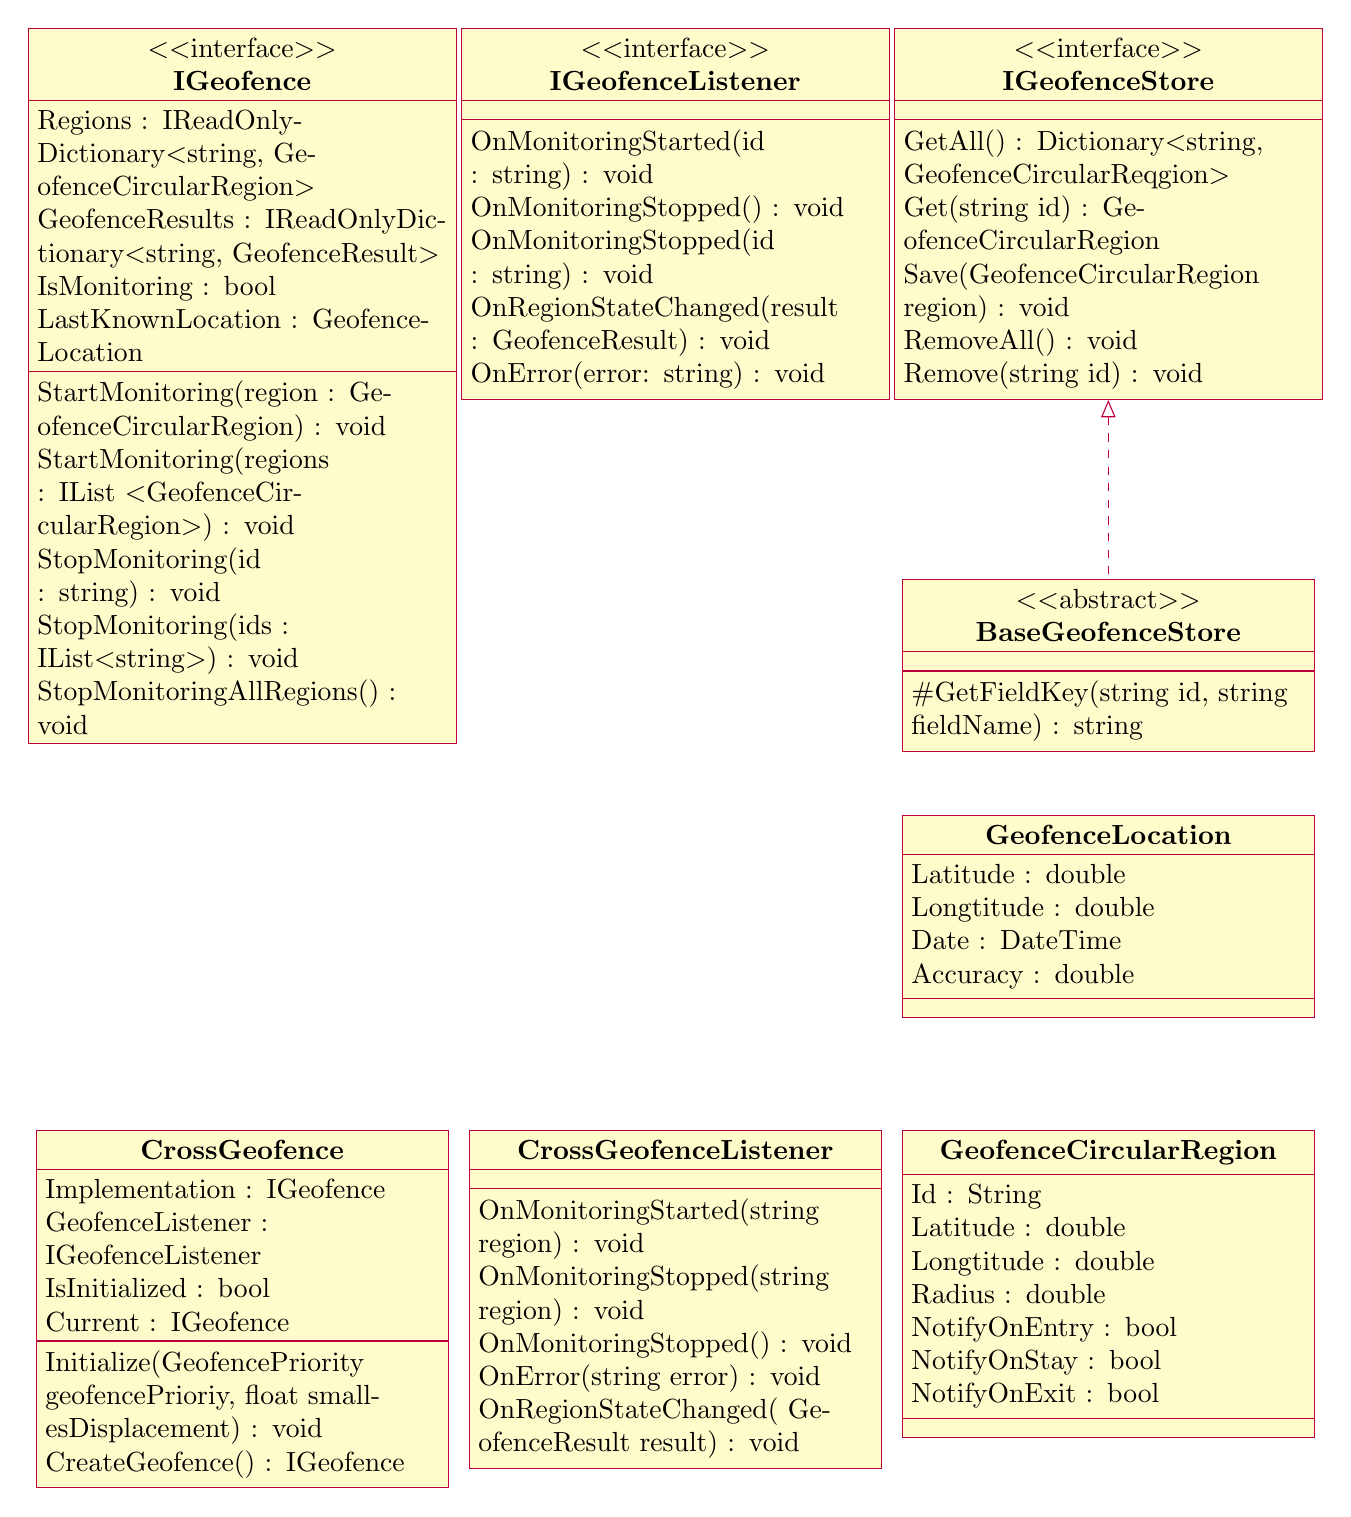
\begin{tikzpicture}
		\begin{class}[text width=5cm]{GeofenceCircularRegion}{11,-14}
			\attribute{Id : String}
			\attribute{Latitude : double}
			\attribute{Longtitude : double}
			\attribute{Radius : double}
			\attribute{NotifyOnEntry : bool}
			\attribute{NotifyOnStay : bool}
			\attribute{NotifyOnExit : bool}
		\end{class}
		
		\begin{class}[text width=5cm]{GeofenceLocation}{11, -10}
			\attribute{Latitude : double}
			\attribute{Longtitude : double}
			\attribute{Date : DateTime}
			\attribute{Accuracy : double}
		\end{class}
		
		\begin{interface}[text width=5.2cm]{IGeofence}{0,0}
			\attribute{Regions : IReadOnlyDictionary\textless string, GeofenceCircularRegion\textgreater}
			\attribute{GeofenceResults : IReadOnlyDictionary\textless string, GeofenceResult\textgreater}
			\attribute{IsMonitoring : bool}
			\attribute{LastKnownLocation : GeofenceLocation}
			\operation{StartMonitoring(region : GeofenceCircularRegion) : void}
			\operation{StartMonitoring(regions : IList \textless GeofenceCircularRegion\textgreater) : void}
			\operation{StopMonitoring(id : string) : void}
			\operation{StopMonitoring(ids : IList\textless string\textgreater) : void}
			\operation{StopMonitoringAllRegions() : void}
		\end{interface}
		
		\begin{class}[text width=5cm]{CrossGeofence}{0,-14}	
			\attribute{Implementation : IGeofence}
			\attribute{GeofenceListener : IGeofenceListener}
			\attribute{IsInitialized : bool}
			\attribute{Current : IGeofence}
			
			\operation{Initialize(GeofencePriority geofencePrioriy, float smallesDisplacement) : void}
			\operation{CreateGeofence() : IGeofence}
		\end{class}
		
		\begin{interface}[text width=5.2cm]{IGeofenceStore}{11,0}
			\operation{GetAll() : Dictionary\textless string, GeofenceCircularReqgion\textgreater}
			\operation{Get(string id) : GeofenceCircularRegion}
			\operation{Save(GeofenceCircularRegion region) : void}
			\operation{RemoveAll() : void}
			\operation{Remove(string id) : void}
		\end{interface}
		
		\begin{abstractclass}[text width=5cm]{BaseGeofenceStore}{11,-7}
			\implement{IGeofenceStore}		
			\operation{\#GetFieldKey(string id, string fieldName) : string}
		\end{abstractclass}
		
		\begin{interface}[text width=5.2cm]{IGeofenceListener}{5.5,0}
			\operation{OnMonitoringStarted(id : string) : void}
			\operation{OnMonitoringStopped() : void}
			\operation{OnMonitoringStopped(id : string) : void}
			\operation{OnRegionStateChanged(result : GeofenceResult) : void}
			\operation{OnError(error: string) : void}
		\end{interface}
		
		\begin{class}[text width=5cm]{CrossGeofenceListener}{5.5,-14}
			\operation{OnMonitoringStarted(string region) : void}
			\operation{OnMonitoringStopped(string region) : void}
			\operation{OnMonitoringStopped() : void}
			\operation{OnError(string error) : void}
			\operation{OnRegionStateChanged( GeofenceResult result) : void}
		\end{class}
\end{tikzpicture}
    \section{Quality management}
This chapter describes the necessary information needed to manage the project quality from the project planning to the delivery
to the customer. Within this document the quality policies, procedures, roles, responsibilities and authorities are defined.\\
At the highest level Quality Management involves planning, doing, checking, and acting to improve project quality standards. Project Quality Management is therefore split into three categories: Quality Planning, Quality Assurance and Quality Control.
\subsection{Organization and Responsibilities}
\begin{table}[htbp]
	\begin{tabular}{ p{4cm} p{3,5cm} p{6,5cm} }
		\textbf{Name} & \textbf{Role} & \textbf{Quality Responsibility} \\ \hline
		Max van der Linden & Project Manager & External communication, Auditing \\ 
		Martijn Bonajo & Configuration Manager & Infrastructure, Source files, Software engineering documentation, Auditing \\ 
		Ron Gebauer & Scrum Master & Scrum planning, Auditing \\ 
		Rene Karoff & Quality Manager & Ensure use of quality guidelines, Auditing \\ 
		Jan Kerkenhoff & Main Engineer & Main Code-Master, Auditing \\
	\end{tabular}
	\caption{Group roles\label{tab:GroupRoles}}
\end{table}

\subsection{Quality Planning}
Since this project is about programming a mobile business application, it is highly important that the system has a minimum of bugs/errors. A good documentation is necessary too, not only because this application will be developed by another SoFa-group after our semester is over, but the customer should understand the system which is developed by us.
\subsubsection{Define Project Quality}
To ensure to quality of the written code it is mandatory to develop every module test-driven, therefore unit-testing is introduced. The written documents will be checked for its grammar, writing style and content.
\subsubsection{Measure Project Quality}
Most of the code of this applicationwas tested, but since we have a lot of GUI related code which we weren't able to do unit tests with, we were not able to achieve the former stated goal of a code coverage of 90\%. 
The code of the application will be tested. Therefore it is a goal to get at least 90\% code coverage, better 100\%. Each evaluation criterion of the written documents will be ranked from “--“ to “++” (“--“ too bad – “++” excellent).
\subsection{Quality Assurance}
Since the code is tested, this will show the group if the quality goal is achieved. Furthermore the written documents will be audited by at least one group member and the project quality manager.
\subsubsection{Analyze Project Quality}
The tool to measure the code coverage \textbf{(which still needs to be defined)} will show the programmer which code is still uncovered, and the writer of a document will receive feedback of the auditing persons, so he can improve on his writing too.
\subsubsection{Improve Project Quality}
To improve the Define proper requirements before starting programming the application.
\subsection{Quality Control}
At the end of the project each deliverable will be audited again, by every team member to ensure the project quality.

    \section{Manual}
\subsection{Credentials}
To continue working on this project you need the following credentials:
\begin{itemize}
\item Access to the Github repository
\item License for Xamarin 
\item Optional: Google Account that contains the API Key
\end{itemize}

\subsection{General setup}
If you want to checkout the project read access to the repository and a trial xamarin license is fine.

\textbf{Important}\\
If you do not have access to the Google account that belongs to the API key used, then you need to exchange the GoogleMaps API Key in the `AndroidManifest.xml`, which is explained in detail later on.

\subsection{Getting the project running}
\begin{itemize}
\item Install Xamarin Studio \url{https://xamarin.com/download}
\item Install Xcode and the latest iOS SDK
\item Install Xamarin Android Player \url{https://xamarin.com/android-player}
\item Download an android device in Xamarin Android Player
\item Install Google Play Services for the emulator \url{https://university.xamarin.com/resources/how-to-install-google-play-on-android-emulator}
\item Checkout git repository
\item Open project in Xamarin Studio
\item  Add your android app fingerprint to the Google Maps API key:
\subitem How to determine your MD5 or SHA1 signature \url{https://developer.xamarin.com/guides/android/deployment,_testing,_and_metrics/MD5_SHA1/}
\subitem This \url{https://developers.google.com/maps/documentation/android-api/signup#get_an_android_api_key} explains how you can add a fingerprint to an existing key or how to create a new key and add it to the app.
\subitem If you want to exchange the key, the android manifest is located at \linebreak \texttt{Droid/Properties/AndroidManifest.xml}
\item  You can now run the project from Xamarin Studio on an emulator

\end{itemize}
 
\subsection{Running on a Device}

\subsubsection{iOS}
\begin{itemize}
\item Get a valid development certificate for iOS development
\item Get a valid provisioning profile for the app including the device you want to run on
\item Connect the device
\item Select the device inside of Xamarin Studio
\item Deploy the app to the device
\end{itemize}
\subsubsection{Android}
\begin{itemize}
\item Connect the device
\item Select the device inside of Xamarin Studio
\item Deploy the app to the device
\end{itemize}


\section{Conclusion}
The TreeWatch app has come a long way but still has a long way to go. A lot of the basic functionality has been implemented. The app can already be used to visualize where all the fields are located on the map and is also able to show overlays such as the block data and biomass.

VAA ICT Consultancy will need to continue the development of the app in order to make it practically usable. This means that a web based database needs to be added which contains all the info. For now the information about the fields is still stored locally on the device. Furthermore also the history and todo parts of the app should be implemented.



    \section{Advice}
Because of performance issues that occur when the app has to calculate the overlays of the fields and the blocks, it is recommended that the server should draw all the polygons and then send it as an image to the phone. Then the phone should be able to overlay this image on the correct position. This would greatly improve the speed of the app.


    \section{Reflection}
\subsection{Max van der Linden}
As the project leader of the SoFa TreeWatch group I learned a lot about what it means to lead a project. This meant that I had to make sure that everyone follows the rules and sticks to the deadlines. One of the tasks of the project leader was also to be the main contacting point to and from the customer. From this I learned a lot about communicating in a professional way.

All in all, in my opinion a good and useful product form which a lot was learned.

\subsection{Martijn Bonajo}

I learned a lot from this project. For me it was the first time creating a multi platform application. This meant learning how to work with Xamarin, using MVVM on the \gls{XamarinForms} and programming to platform specific \gls{api}s.\\
As configuration manager I was responsible for making sure everyone could run all the software that was needed during the project.

\subsection{Rene Karoff}


\subsection{Jan Kerkenhoff}


\subsection{Ron Gebauer}
In this project I learn a bunch of stuff. As an example I worked the first time with \gls{XamarinStudio} and was a part in the creation of an cross platform application. Furthermore I learned a lot from our customer, which creates an really interesting atmosphere inside the meetings. In addition to that I got more and more confirm with \gls{scrum}, which was our \gls{AgileSoftwareDevelopment} method.

Finally I will say that this \gls{sofa} one of the most interesting and helping modules was in my study.
    %\include{pages/appendix}

    \clearpage
    \bibliographystyle{plain}
    \bibliography{biblist}

\end{document}
